\section{Wojciech pacholczak}

Jest zdjecie kotka (see Figure~\ref{fig:cat}).


\begin{figure}[htbp]
\centering
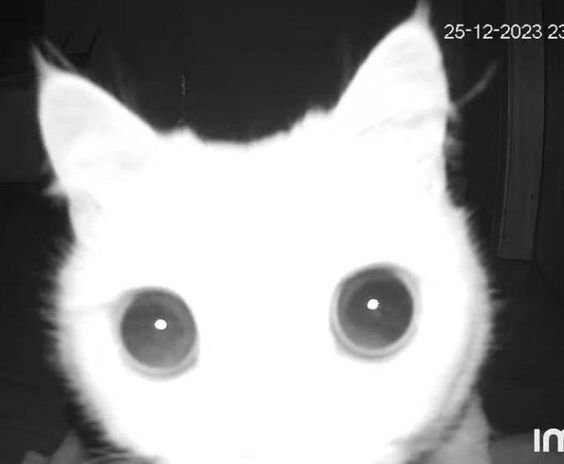
\includegraphics[width=0.4\textwidth]{pictures/bigEyedCat.jpg} \
\caption{This cat is looking.}
\label{fig:cat}
\end{figure}

Tabela~\ref{tab:words} ma w sobie losowe słowa

\begin{table}[htbp]
\centering
\begin{tabular}{|l|l|l|l|l|}
\hline
rumbling       & kolumna & tez & i tutaj                & poruszenie \\ \hline
\textbf{kolos} & 1       & 3   & \textbf{opancerzony}   & 123        \\ \hline
1              & 3221    & 32  & \textbf{szczekowy}     & 22352      \\ \hline
7              & 2       & 1   & \multicolumn{1}{c|}{1} & 3          \\ \hline
\end{tabular}
\label{tab:words}
    \caption{Słowa.}
\end{table}

\begin{itemize}
   \item Idziemy dalej
   \begin{itemize}
     \item I dalej
     \begin{itemize}
       \item I dalej
       \begin{itemize}
         \item I tu koniec
       \end{itemize}
     \end{itemize}
   \end{itemize}
 \end{itemize}


\begin{enumerate}
  \item To moja lista.
  \item Działa.
\end{enumerate}


wzór eulera:
$e^{i\pi} - 1 = 0$
\vspace{0.5cm}

 Lorem ipsum dolor sit amet, consectetur adipiscing elit. Fusce nec nunc eu sapien tristique faucibus. Vivamus sagittis pulvinar est ac viverra. Etiam varius odio sapien, at posuere nulla \textbf{tristique ac.} Nulla nec mattis justo. Nunc sollicitudin finibus ipsum, at volutpat dolor gravida a. Quisque tristique venenatis erat dapibus auctor. Sed sit amet euismod tellus. Aenean facilisis felis eget fermentum \underline{tempus.}  Nunc pulvinar finibus mauris, non luctus purus efficitur ultrices. Proin aliquet eros metus, sed finibus magna sollicitudin in.

Lorem ipsum dolor sit amet, consectetur adipiscing elit. Aliquam vel vehicula magna, ut egestas magna. Praesent bibendum porta ullamcorper. Donec eu hendrerit purus, quis venenatis enim. Sed aliquet erat nec ipsum aliquet, et mattis odio posuere. In ut massa tellus. Proin nec consequat purus. Nulla maximus, urna et sodales tempor, est quam luctus metus, at cursus massa erat ut nunc. Sed interdum aliquet ultricies. Curabitur arcu odio, venenatis eget pharetra eu, varius quis erat. Proin libero leo, commodo in ex in,\textbf{\textit{egestas blandit est}} . Suspendisse interdum purus purus, sed dapibus velit accumsan nec. Ut vel turpis at eros scelerisque ullamcorper et et massa.